% document formatting
\documentclass[10pt]{article}
\usepackage[utf8]{inputenc}
\usepackage[left=1in,right=1in,top=1in,bottom=1in]{geometry}
\usepackage[T1]{fontenc}
\usepackage{xcolor}

% math symbols, etc.
\usepackage{amsmath, amsfonts, amssymb, amsthm}

% lists 
\usepackage{enumerate}

% images
\usepackage{graphicx} % for images
\usepackage{tikz}

% code blocks
\usepackage{minted, listings} 

% verbatim greek
\usepackage{alphabeta}
\DeclareMathOperator*{\argmin}{arg\,min}
\DeclareMathOperator*{\argmax}{arg\,max}

\graphicspath{{./assets/images/}}

\title{02-620 Week 4 \\ \large{Machine Learning for Scientists}}
 
\author{Aidan Jan}

\date{\today}

\begin{document}
\maketitle

\section*{Logistic Regression}
Logistic regression aims to fit a logistic curve to data.
\[P(Y_i = 1 | x_i; \theta) = \frac{1}{1 + e^{-(\theta_0 + \theta_1 x_i)}}\]
The linear part in the exponent is the equation for the decision boundary.

\subsection*{Logistic Regression: Data}
\begin{itemize}
	\item $N$ data points with $D$ features: $x_i \in \mathbb{R}^D$
	\item Labels: $y_i \in \{0, 1\}$
\end{itemize}
\subsection*{Logistic Regression: Model}
\begin{itemize}
	\item Parameters: $\theta = (\theta_0, \theta_1, \cdots, \theta_D)$
	\item Linear predictor: $\mu(x) = \theta_0 + \sum_{j = 1}^D \theta_j x_j$
	\item Sigmoid: $\sigma(t) = \frac{1}{1 + e^{-t}}$
	\item Parametric function:
	\[P(Y = 1 | x; \theta) = \frac{1}{1 + \exp\left(-\left(\theta_0 + \sum_{j = 1}^D \theta_j x_j\right)\right)} = \sigma(\mu(x)) = \frac{1}{1 + e^{-\mu(x)}}\]
\end{itemize}
We can find $P(Y = 0 | x; \theta)$ by subtracting the $Y = 1$ case from 1 since the probabilities must sum to 1.
\[P(Y = 0 | x; \theta) = 1 - \sigma(\mu(x)) = \frac{e^{-\mu(x)}}{1 + e^{-\mu(x)}}\]

\subsubsection*{Logistic Function (Sigmoid)}
\begin{center} 
	\includegraphics*[width=0.5\textwidth]{W3_1.png} 
\end{center}
\begin{itemize}
	\item When $t = 0$, $\sigma(t) = 0.5$
	\item When $t \rightarrow \infty$, $\sigma(t) = 1$
	\item When $t \rightarrow -\infty$, $\sigma(t) = 0$
\end{itemize}

\subsection*{Simple Classifier vs. Logistic Classifier}
\begin{center} 
	\includegraphics*[width=0.7\textwidth]{W3_2.png} 
\end{center}
Typically, when the logistic function is used for classification, we round the value to the nearest integer.  However, the logistics curve is useful because the curve is differentiable, which makes gradient descent possible.

\subsection*{Decision Boundary in Logistic Regression}
\begin{center} 
	\includegraphics*[width=0.5\textwidth]{W3_3.png} 
\end{center}
We know that the probability of the class label $Y = 1$ and $Y = 0$ are:
\begin{align*}
P(Y = 1 | x; \theta) &= \frac{1}{1 + e^{-\mu(x)}}
P(Y = 0 | x; \theta) &= 1 - \sigma(\mu(x)) = \frac{e^{-\mu(x)}}{1 + e^{-\mu(x)}}
\end{align*}
Therefore, 
\[\frac{P(Y = 1 | x; \theta)}{(Y = 0 | x; \theta)} = e^{\mu(x)}\]
We can log both sides to get
\[\mu(x) = \log \left(\frac{P(Y = 1 | x; \theta)}{(Y = 0 | x; \theta)}\right)\]
Notice that $\mu(x)$ is a linear model!  $\mu(x) = \theta_0 + \sum_{j = 1}^D \theta_j x_j = 0$

\subsection*{Logistic Regression: Beyond Binary Classification}
\textbf{Data}
\begin{itemize}
	\item $N$ data points with $D$ features: $x_i \in \mathbb{R}^D$
	\item Labels: $y_i \in \{1, \cdots, K\}$
\end{itemize}
\textbf{Model}
\begin{itemize}
	\item Parameters: $\theta = (\theta_{k0}, \theta_{k1}, \cdots, \theta_{kD})$, for $k = 1, \dots, K - 1$
	\item Linear predictor: $\mu_k(x) = \theta_{k0} + \sum_{j = 1}^D \theta_{kj} x_j$, for $k = 1, \dots, K - 1$
	\item Sigmoid: $\sigma(t) = \frac{1}{1 + e^{-t}}$
	\item Parametric function:
	\begin{itemize}
	    \item For $k = 1, \dots, K - 1$, $P(Y = k | x; \theta) = \sigma(\mu_k (x)) = \frac{e^{-\mu_k(x)}}{1 + \sum_{k = 1}^{K - 1} e^{-\mu_k(x)}}$
	    \item $P(Y = K | x; \theta) = \frac{1}{1 + \sum_{k = 1}^{K - 1} e^{-\mu_k(x)}}$
	    \item Note that $\sum_{k = 1}^K P(Y = k | x; \theta) = 1$.
    \end{itemize}
\end{itemize}

\subsection*{Logistic Regression: Inference}
For a new data point $x_{i'}$, predict $\hat{y}_{i'} = f(x_{i'}; \hat{\theta})$\\
Compute and classify accordingly:
\begin{itemize}
	\item $P(Y = 1 | x; \theta) = \sigma(\mu(x))$
	\item $P(Y = 0 | x; \theta) = 1 - \sigma(\mu(x))$
\end{itemize}

\subsection*{Logistic Regression: Learning via MLE}
\begin{itemize}
	\item \textbf{Data:} $\mathcal{D} \::\: x_1, \cdots, x_N \in \mathbb{R}^D$, $y_1, \cdots, y_N \in \{0, 1\}$
	\item \textbf{Estimate parameters:} $\theta = (\theta_0, \theta_1, \cdots, \theta_D)$
	\item \textbf{MLE estimate:} $\hat{\theta} = \argmax_\theta \sum_{i = 1}^N \log P(Y_i | x_i; \theta) = \argmax_\theta l(\theta)$
\end{itemize}
\begin{align*}
    l(\theta) &= \sum_{i = 1}^N [Y_i \log P(Y_i = 1 | x_i; \theta) + (1 - Y_i) \log P(Y_i = 0 | x_i; \theta)] \\
    &= \sum_{i = 1}^N \left[Y_i \log \frac{P(Y_i = 1 | x_i;\theta)}{P(Y_i = 0 | x_i; \theta)} + \log P(Y_i = 0 | x_i; \theta)\right] \\
    &= \sum_{i = 1}^N \left[Y_i \left(\theta_0 + \sum_{j = 1}^D \theta_j x_{ij}\right) - \log\left(1 + \exp \left(\theta_0 + \sum_{j = 1}^D \theta_j x_{ij}\right)\right)\right] \\
    \intertext{Take derivative of $l(\theta)$ with respect to $\theta$}
    \frac{\partial l(\theta)}{\partial \theta_0} &= \sum_{i = 1}^N \left[Y_i - \frac{e^{\mu_i}}{1 + e^{\mu_i}}\right] \\
    \frac{\partial l(\theta)}{\partial \theta_j} &= \sum_{i = 1}^N x_{ij} \left[Y_i - \frac{e^{\mu_i}}{1 + e^{\mu_i}}\right] \quad \text{for } j = 1, \dots, D
\end{align*}
Note that
\begin{itemize}
	\item $l(\theta)$ is concave
	\item Gradient ascent/descent gives the optimal solution.
\end{itemize}
To gradient ascent,
\begin{itemize}
	\item For $t = 1, 2, \dots$:
	\begin{itemize}
	    \item For all $j$, update $\theta_j \leftarrow \theta_j + \Delta \frac{\partial l(\theta)}{\partial \theta_j}$  ($\Delta$ is the step size or learning rate.)
    \end{itemize}
    \item Stop when $\left|l(\theta^{(t)}) - l(\theta^{(t - 1)})\right| < \epsilon$
    \item $\epsilon$ is a small value (error).
\end{itemize}

\subsubsection*{Aside: Gradient Ascent}
To find $x$ that maximizes a function $f(x)$:
\begin{itemize}
	\item Start with random initialization $x_0$
	\item For $t = 1, \dots$
	\begin{itemize}
	    \item $x_{t + 1} = x_t + \lambda f'(x_t)$ with step size $\lambda$
    \end{itemize}
    \item $\lambda$
    \begin{itemize}
	    \item $\lambda \uparrow$: overshoot
	    \item $\lambda \downarrow$: too many iterations.
    \end{itemize}
\end{itemize}
\begin{center} 
	\includegraphics*[width=0.7\textwidth]{W3_4.png} 
\end{center}
Log-likelihood of the logistic regression is concave.  Gradient descent/ascent will:
\begin{itemize}
	\item reach the maximum of the log likelihood
	\item find the optimal estimate of the parameters
\end{itemize}

\subsection*{Logistic Regression: Adding Regularization}
\begin{itemize}
	\item \textbf{MLE estimate}
	\[\hat{\theta} = \argmax_\theta \sum_{i = 1}^N \log P(Y_i | x_i; \theta)\]
	\item \textbf{Ridge regression}
	\[\hat{\theta} = \argmax_\theta \sum_{i = 1}^N \log P(Y_i | x_i; \theta) + \lambda \Vert \theta \Vert_2^2\]
	\item \textbf{LASSO regression}
	\[\hat{\theta} = \argmax_\theta \sum_{i = 1}^N \log P(Y_i | x_i; \theta) + \lambda \Vert \theta \Vert_1\]
\end{itemize}

\subsection*{Inseparable Distributions}
Recall that
\[P(Y = 1 | x; \theta) = \frac{1}{1 + \exp \left(-\left(\theta_0 + \sum_{j = 1}^D \theta_j x_j\right)\right)}\]
What if positive and negative samples are not completely separable?
\begin{center} 
	\includegraphics*[width=0.6\textwidth]{W4_1.png} 
\end{center}
\begin{itemize}
	\item How would logistic regression handle this?
	\item Limitations of logistic regression?
\end{itemize}

\subsubsection*{Generative vs. Discriminative Classifiers}
Training classifiers involves estimating $f \::\: X \rightarrow Y$ or $P(Y | X)$.
\begin{itemize}
	\item \textbf{Generative Classifiers} (e.g., Naive Bayes)
	\begin{itemize}
	    \item Model and learn $P(Y, X) = P(X | Y) P(Y)$
	    \item Derive $P(Y | X)$ from $P(Y, X)$ using Bayes rule
	    \item Find $\theta = \argmax_\theta \prod_i P(y_i, x_i | \theta)$
	    \item Different assumptions about \textit{generative process} for the data: $P(X, Y)$, priors on $\theta, \dots$.
    \end{itemize}
	\item \textbf{Discriminative classifiers} (e.g., Logistic regression)
	\begin{itemize}
	    \item Model $P(Y|X)$ directly
	    \item Find $\theta = \argmax_\theta \prod_i P(y_i | x_i, \theta)$
	    \item Different assumptions about conditional probability: $P(Y | X)$, priors on $\theta, \dots$ 
    \end{itemize}
\end{itemize}

\subsection*{Measuring Accuracy of Classifier}
\begin{itemize}
	\item Precision = (number classified as positive AND positive in data) / (number classified as positive)
	\begin{itemize}
	    \item e.g., how many of the patients classified as ``disease'' are in fact truly ``disease''?
    \end{itemize}
    \item Recall = (number classified as positive AND positive in data) / (number ground truth positive in data)
    \begin{itemize}
	    \item e.g., how many of the ``disease'' patients were classified as ``disease''?
    \end{itemize}
    \item True positive (classified as positive, positive in data)
    \item False positive (classified as positive, negative in data)
    \item True negative (classified as negative, negative in data)
    \item False negative (classified as negative, positive in data)
\end{itemize}

\subsection*{Summary}
\begin{itemize}
	\item Naive Bayes Classifier
	\begin{itemize}
	    \item Model description via $P(X | Y)$ and $P(Y)$
	    \item MLE: closed-form solution, no iterative learning
    \end{itemize}
    \item Logistic regression
    \begin{itemize}
	    \item Model description for $P(Y | X)$
	    \item MLE: no closed-form solution, iterative learning via gradient descent
    \end{itemize}   
    \item Generative vs. Discriminative classifier
\end{itemize}

\section*{Decision Trees}
\textbf{Data}
\begin{itemize}
	\item $N$ data points with $D$ attributes: $x_i$ (discrete / continuous / mixed)
	\item Labels: $y_i \in \{0, 1\}$
\end{itemize}
For example:
\begin{center}
    \begin{tabular}{c|c|c|c|c|c}
    Day & Outlook & Temperature & Humidity & Wind & PlayTennis (Label) \\ \hline
    1 & Sunny & Hot & High & Weak & No \\
    2 & Sunny & Hot & High & Strong & No \\
    3 & Overcast & Hot & High & Weak & No \\
    4 & Rain & Mild & High & Weak & Yes \\
    5 & Rain & Cool & Normal & Weak & Yes \\
    6 & Rain & Cool & Normal & Strong & No \\
    7 & Overcast & Cool & Normal & Strong & Yes \\
    8 & Sunny & Mild & High & Weak & No \\
    9 & Sunny & Cool & Normal & Weak & Yes \\
    10 & Rain & Mild & Normal & Weak & Yes \\
    11 & Sunny & Mild & Normal & Strong & Yes \\
    12 & Overcast & Mild & High & Strong & Yes \\
    13 & Overcast & Hot & Normal & Weak & Yes \\
    14 & Rain & Mild & High & Strong & No
    \end{tabular}
\end{center}
\textbf{Model}
\begin{itemize}
	\item Each \textbf{internal node} selects an attribute $x_j$ and applies a decision rule (e.g., $x_j = v$ for discrete or $x_j < \tau$ for continuous features)
	\item Each \textbf{branch} corresponds to an outcome of the rule
	\item Each \textbf{leaf node} outputs a prediction: a class label or $P(Y | x \in leaf)$
\end{itemize}
\begin{center}
    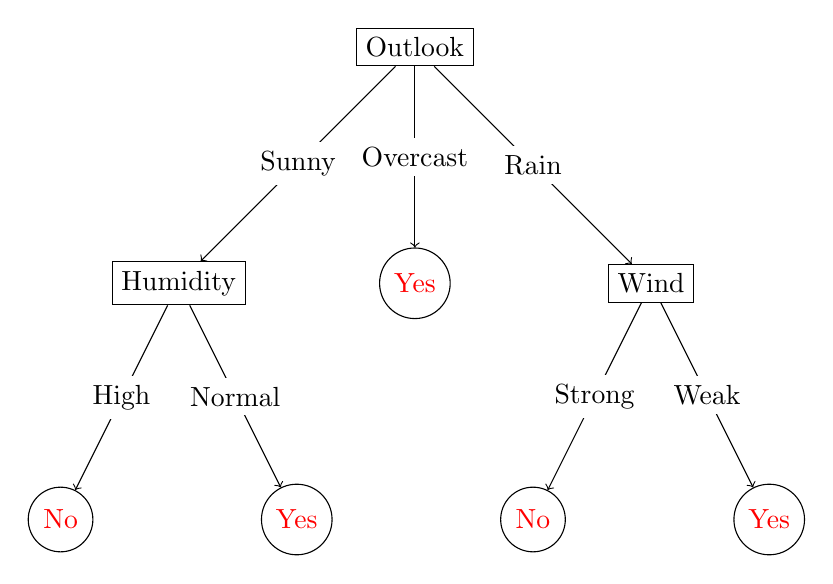
\begin{tikzpicture}
        \node[draw] at (0, 0) (a1) {Outlook};
        \node[draw] at (-3, -3) (b1) {Humidity};
        \node[draw, circle] at (0, -3) (b2) {\textcolor{red}{Yes}};
        \node[draw] at (3, -3) (b3) {Wind};
        \node[draw, circle] at (-4.5, -6) (c1) {\textcolor{red}{No}};
        \node[draw, circle] at (-1.5, -6) (c2) {\textcolor{red}{Yes}};
        \node[draw, circle] at (1.5, -6) (c3) {\textcolor{red}{No}};
        \node[draw, circle] at (4.5, -6) (c4) {\textcolor{red}{Yes}};

        \draw[->] (a1) -- node[midway, fill=white] {Sunny} (b1);
        \draw[->] (a1) -- node[midway, fill=white] {Overcast} (b2);
        \draw[->] (a1) -- node[midway, fill=white] {Rain} (b3);
        \draw[->] (b1) -- node[midway, fill=white] {High} (c1);
        \draw[->] (b1) -- node[midway, fill=white] {Normal} (c2);
        \draw[->] (b3) -- node[midway, fill=white] {Strong} (c3);
        \draw[->] (b3) -- node[midway, fill=white] {Weak} (c4);
    \end{tikzpicture}
\end{center}
\textbf{Inference}
\begin{itemize}
	\item For a new data point, traverse the tree from the root to a leaf to obtain the prediction
    \item Day 1 $\rightarrow$ No (Outlook: Sunny $\rightarrow$ Humidity: High $\rightarrow$ No).
\end{itemize}

\subsection*{Decision Tree Motivations}
\begin{itemize}
	\item Can produce small, accurate, and interpretable classifiers
	\item Often provide insight into the problem and help debug features
	\item Naturally captures feature interactions (e.g., "sunny AND humid") - interactions that linear models miss.
	\item Fast and cheap at test time - not all features need to be computed
	\item Can account for feature acquisition costs - some features are much cheaper than others (e.g., "blood pressure" vs. "MRI")
\end{itemize}

\subsection*{Decision Tree Learning}
\begin{itemize}
	\item Estimate internal nodes and decision rules for the decision tree
    \item \textbf{Initialize:} assign all data points to the root node.
    \item \textbf{Recursively grow the tree.}  For data points at the current node, select the best \textbf{attribute} $x_j$ and split:
    \begin{itemize}
	    \item Categorical: $x_j = c_1, c_2, \dots$
	    \item ContinuousL $x_j < \tau$ or $x_j \geq \tau$
    \end{itemize}
    \item Ask: Does $x_j$ help predict $y$?  (e.g., lower the \textbf{entropy} of $y$ in the resulting partitions (details later).)
    \item Assign data points to corresponding child nodes, repeat until a node is sufficiently homogeneous, and make the node a leaf and assign majority label.
\end{itemize}
Common stopping criteria include:
\begin{itemize}
	\item Entropy (or Gini) below a threshold
	\item Maximum tree depth reached
	\item Minimum node size reached
\end{itemize}
\textbf{Procedure:}
For each attribute $x_1, \dots, x_D$, evaluate the \textbf{entropy} of the resulting splits.  Select the one with the most entropy reduction.

\subsection*{Entropy}
Entropy measures impurity in a set of points.  The lower the entropy, the more pure the data is.
\begin{itemize}
	\item For example, consider the decision for \textit{PlayTennis} above.  If we originally tested for Humidity instead of Outlook, then we have
	\begin{itemize}
	    \item [3+, 4-] (E = 0.985) if humidity is high
	    \item [6+, 1-] (E = 0.592) if humidity is normal
    \end{itemize}
    \item $+$ represents the count of "Yes" for \textit{PlayTennis}, and $-$ represents the count for "No" for \textit{PlayTennis}
    \item The more the counts lean to one direction, the lower the entropy.  Therefore, if every label is "Yes" or if every label is "No", then the entropy is 0.
    \item On the contrary, equal counts in "Yes" and "No" lead to an entropy of $1$, the maximum value of entropy possible.
\end{itemize}
Entropy is represented by a distribution.  
\begin{itemize}
	\item \textbf{Binary distribution:} If $Y \sim Bern(p)$, then $H(Y) = -p \log_2 p - (1 - p) \log_2 (1 - p)$.
	\item \textbf{Discrete distribution:} If $Y$ takes values $\{c_1, \dots, c_K\}$ with probabilities $p_1, \dots, p_k$, then $H(y) = -\sum_{k_1}^K p_k \log_2 p_k$
    \item \textbf{Sample entropy (binary labels):} For a set of data points $S$, let $p_0$ and $p_1$ be the proportion of 0's and 1's.  Then $H(S) = -p_0 \log_2 p_0 - p_1 \log_2 p_1$
\end{itemize}

\subsection*{Conditional Entropy and Information Gain}
For discrete random variables $X$ and $Y$, the entropy $H(Y) = \sum_y P(Y = y) \log_2 P(Y = y)$ quantifies the uncertainty of a random variable $Y$.\\\\
\begin{itemize}
	\item \textbf{Conditional entropy:} $H(Y|X) = \sum_x P(X = x) H(Y | X = x)$ quantifies the \textit{remaining uncertainty} of $Y$ after knowing $X$.
	\item \textbf{Information gain:} $IG(Y; X) = H(Y) - H(Y | X)$ quantifies the reduction in uncertainty due to knowing $X$.
\end{itemize}
\subsubsection*{Example}
For a dataset $S$, let $p_0$ and $p_1$ be the proportion of 0's and 1's.  Partition of $S$ into $S_0$ and $S_1$ with proportions $\pi_0$ and $\pi_1$.
\begin{itemize}
	\item Let $p_{00}$ and $p_{01}$ be the proportion of 1's and 0's in $S_0$
	\item Let $p_{10}$ and $p_{11}$ be the proportion of 1's and 0's in $S_1$
\end{itemize}
\begin{center} 
	\includegraphics*[width=\textwidth]{W4_2.png} 
\end{center}
\textbf{Entropy:}
\begin{align*}
    H(S) &= -p_0 \log_2 p_0 - p_1 \log_2 p_1 \\
    H(S_0) = -\frac{4}{7} \log_2 \frac{4}{7} - \frac{3}{7} \log_2 \frac{3}{7} = 0.985 \\
    H(S_1) = -\frac{1}{7} \log_2 \frac{1}{7} - \frac{6}{7} \log_2 \frac{6}{7} = 0.592
\end{align*}
\textbf{Conditional Entropy:}
\begin{align*}
    H(S | partition) &= \pi_0 H(S_0) + \pi_1 H(S_1) = -\pi_0 (p_0 \log_2 p_{00} - p_1 \log_2 p_{01}) - \pi_1 (p_0 \log_2 p_{10} - p_1 \log_2 p_{11}) \\
    &= -\frac{7}{14} \cdot 0.985 - \frac{7}{14} 0.592 = 0.788
\end{align*}
quantifies the remaining uncertainty of $S$ after knowing the partition.\\\\
\textbf{Information gain:}
\begin{align*}
    IG(S | partition) &= H(S) - H(S | partition) \\
    &= 0.94 - 0.788 = 0.152
\end{align*}
quantifies the reduction in uncertainty due to knowing the partition.\\\\
We want the attribute with the largest information gain.

\subsection*{Decision Tree Can Completely Overfit the Data}
\begin{itemize}
	\item Decision trees can be grown arbitrarily deep to achieve zero training error.
	\item However, overly complex trees may not generalize well.
\end{itemize}
Recall that overfitting occurs if:
\begin{itemize}
	\item Error(training data) is low, and
	\item Error(All data) is high.
\end{itemize}
How to avoid overfitting:
\begin{itemize}
	\item Stop growing the tree when the data split is not statistically significant
	\item Growing tree only to a given depth
	\item Grow full tree then prune
	\item \textbf{Split the data into training and test sets.}  Evaluate the tree on the test set, but train on the training set.
\end{itemize}
How to select the best tree
\begin{itemize}
	\item Should we use the training data or test data to measure the classification accuracy of the decision tree?
\end{itemize}

\subsection*{Decision Trees with Continuous Attributes}
Suppose for our \textit{PlayTennis} example, we now want to consider temperature.  To do this, we \textbf{learn a decision threshold $\tau$.}
\begin{itemize}
	\item Sort the sample values
	\item Evavluate all candidate thresholds that produce distinct splits
	\item Select the threshold with the highest information gain
	\item Complexity $O(N_{node})$
\end{itemize}
The decision boundary may be decided using other models, for example logistic regression.  Alternatively, we can just section out the points like follows:
\subsubsection*{What's the decision boundary for decision trees (red dots vs. rest)?}
\begin{center} 
	\includegraphics*[width=\textwidth]{W4_3.png} 
\end{center}
In this case, even just for two labels, the decision boundary is very complicated.

\subsection*{Decision Tree Pros and Cons}
\begin{itemize}
	\item Pros:
	\begin{itemize}
	    \item Tree structure: easy to interpret
	    \item Handle mixed discrete and continuous inputs
	    \item Automatic variable selection
	    \item Scale well to large data
    \end{itemize}
	\item Cons:
	\begin{itemize}
	    \item Prediction accuracy is often lower than other classifiers
	    \item Small changes in data have a large change on the tree structure (called \textbf{high variance})
        \item An error at the top of the tree affect the rest of the tree growing process
    \end{itemize}
\end{itemize}

\subsection*{Decision Tree Classifier Summary}
\begin{itemize}
	\item Model:
	\begin{itemize}
	    \item Tree-structured, non-linear model
    \end{itemize}
	\item Learning:
	\begin{itemize}
	    \item Recursively grow the tree
	    \item Select attributes and splits based on information gain
	    \item Prune the tree to avoid overfitting
    \end{itemize}   
	\item Inference:
	\begin{itemize}
	    \item Traverse the tree to make predictions
	    \item Computationally efficient at test time
    \end{itemize}
\end{itemize}
\end{document}